\documentclass[pscyr,notitle]{hedwork}
\usepackage[russian]{babel}
\usepackage{graphicx}
\usepackage{setspace}
\usepackage{hyperref}
\usepackage{listings}
\graphicspath{{images/}}

\lstset{
    extendedchars=\true,
    inputencoding=utf8
}

\lstdefinelanguage{js}{
  keywords={break, case, catch, continue, debugger, default, delete, do, else, finally, for, function, if, in, instanceof, new, return, switch, this, throw, try, typeof, var, void, while, with},
  morecomment=[l]{//},
  morecomment=[s]{/*}{*/},
  morestring=[b]',
  morestring=[b]",
  sensitive=true,
  basicstyle=\small,
}

\renewcommand{\thesection}{\arabic{section}.}
\renewcommand{\thesubsection}{\thesection\arabic{subsection}.}
\renewcommand{\thesubsubsection}{\thesubsection\arabic{subsubsection}.}

\newcommand{\maketitlepage}{
    \begin{titlepage}
        \singlespacing
        \newpage
        \begin{center}
            Министерство образования и науки Российской Федерации \\
            Федеральное государственное бюджетное образовательное \\
            учреждение высшего профессионального образования \\
            <<Волгоградский государственный технический университет>> \\
            Факультет электроники и вычислительной техники\\
            Кафедра физики
        \end{center}
        \vspace{9em}
        \begin{center}
            Лабораторная работа\\[.5em]
            \Large\scshape <<>>
        \end{center}
        \vspace{1em}        
        \begin{center}
            Методические указания
        \end{center}
        \vspace{3em}
        
        \vspace{\fill}
        \begin{center}
            Волгоград, \the\year
        \end{center}

    \end{titlepage}
    \setcounter{page}{2}
}

\begin{document}
    \maketitlepage
    \begin{frame}
    \frametitle{Содержание}
    \tableofcontents
\end{frame}

\section{Введение}
\begin{frame}
    \frametitle{OpenStreetMap}
    \begin{minipage}[h]{0.20\textwidth}
        \begin{figure}[ht!]
            
\includegraphics[width=\textwidth]{osm-logo}
        \end{figure}
    \end{minipage}
    \begin{minipage}[h]{0.78\textwidth}
        \textbf{OpenStreetMap} -- некоммерческий веб-картографический проект, который создает и 
        предоставляет свободные географические данные и возможность создавать карты всего мира 
        кому угодно, кто это хочет.
    \end{minipage}

    \begin{figure}[ht!]
        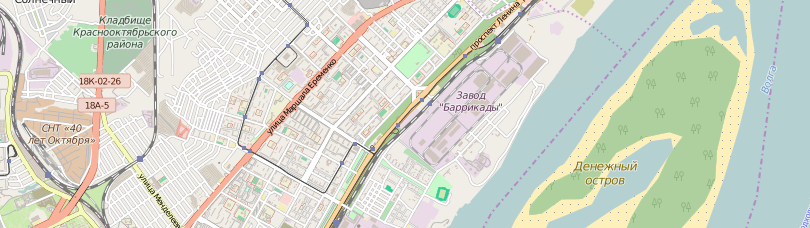
\includegraphics[width=\textwidth]{osm-map}
    \end{figure}

    \scriptsize\begin{itemize}
        \item \url{http://openstreetmap.org}
        \item \url{http://openstreetmap.ru}
    \end{itemize}\normalsize
\end{frame}

\section{Возможности}
\begin{frame}
    \frametitle{Возможности платформы}
    Проект обладает большими функциональными возможностями. От свободных 
    картографических данных, до разработки программного обеспечения на основе OSM.
    
    Некоторые из них:
    \begin{itemize}
        \item охватывает всю поверхность земного шара
        \item создание сервисов на основе данных OSM
        \item экспорт карт в форматы PNG, JPEG, SVG, PDF, PostScript
        \item инструменты и сервисы
    \end{itemize}
\end{frame}

\section{Формат данных}
\begin{frame}
    \frametitle{Структура данных OpenStreetMap}
    \begin{figure}[ht!]
        \center
        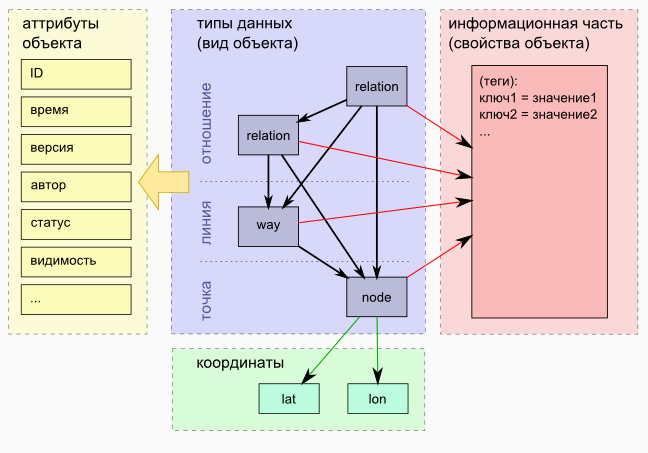
\includegraphics[width=0.8\textwidth]{p1}
    \end{figure}
    \scriptsize
    \begin{itemize}
        \item формат данных в WGS84
        \item использование проекции Меркатора\footnotemark
    \end{itemize}
    \normalsize
    \footnotetext{\scriptsize\url{https://en.wikipedia.org/wiki/Mercator_projection}}
\end{frame}

\section{Базовые типы}
\begin{frame}[fragile]
    \frametitle{Node, way}
    \textbf{Node (\emph{точка})} -- это минимальный набор данных, который содержит в себе 
    информацию о паре координат: широта, долгота.
    \begin{lstlisting}
<node id='42' lat='48.714' lon='44.52834 />
    \end{lstlisting}
    \textbf{Way (\emph{линия})} -- это совокупность указателей на объекты типа \textbf{node}.
    \begin{lstlisting}
<node id='42' lat='48.71400' lon='44.52834' />
<node id='43' lat='48.71475' lon='44.52651' />
<way id='88'>
  <nd ref='42' />
  <nd ref='43' />
</way>
    \end{lstlisting}
\end{frame}

\begin{frame}[fragile]
    \frametitle{Relation, tag}
    \textbf{Relation (\emph{отношение})} -- группы точек, линий и других отношений, которым 
    назначаются некоторые свойства.
    \begin{lstlisting}
<relation id='128'>
  <member type='way' ref='88' />
  <member type='node' ref='42' />
</relation>
    \end{lstlisting}
    \textbf{Tag (\emph{ярлык})} -- пары <<ключ -- значение>>, могут назначаться точкам, 
    линиям и отношениям.
    \begin{lstlisting}
<node id="365500652" visible="true" version="2" changeset="29181889"
  timestamp="2015-03-01T17:22:48Z" user="b108" uid="621253"
  lat="48.7855571" lon="44.5668745">
    <tag k="amenity" v="clinic"/>
    <tag k="name" v="Детская поликлиника"/>
</node>
    \end{lstlisting}
\end{frame}

\section{Информационная схема объектов}
\begin{frame}[fragile]
    \frametitle{Представление объектов}
    \begin{lstlisting}
<node id="1086155180" visible="true" version="2" changeset="14350424"
  timestamp="2012-12-21T02:36:20Z" user="sashayohan" uid="377222"
  lat="48.7908860" lon="44.5967542">
    <tag k="amenity" v="fuel"/>
    <tag k="brand" v="Газпром"/>
    <tag k="fuel:cng" v="no"/>
    <tag k="fuel:lpg" v="yes"/>
    <tag k="name" v="АГЗС"/>
</node>
...
<node id="365500652" visible="true" version="2" changeset="29181889"
  timestamp="2015-03-01T17:22:48Z" user="b108" uid="621253"
  lat="48.7855571" lon="44.5668745">
    <tag k="amenity" v="clinic"/>
    <tag k="name" v="Детская поликлиника"/>
</node>
...
<node id="1112947371" visible="true" version="2" changeset="33330865"
  timestamp="2015-08-14T08:03:34Z" user="avkuzmin" uid="305458"
  lat="48.7843512" lon="44.5647101">
<tag k="crossing" v="traffic_signals"/>
    \end{lstlisting}
\end{frame}

\section{Геометрические примитивы}
\subsection{Point}
\begin{frame}
    \frametitle{Point}
    \textbf{Point (\emph{точка})} -- это один объект типа \emph{node}.
    \begin{figure}[ht!]
        \center
        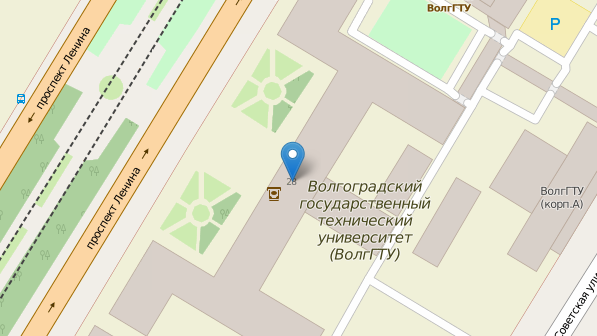
\includegraphics[width=\textwidth]{point}
    \end{figure}
\end{frame}

\subsection{Line}
\begin{frame}
    \frametitle{Line}
    \textbf{Line (\emph{линия})} -- соответствует объекту типа \emph{way}, 
    содержащему два объекта \emph{node}.
    \begin{figure}[ht!]
        \center
        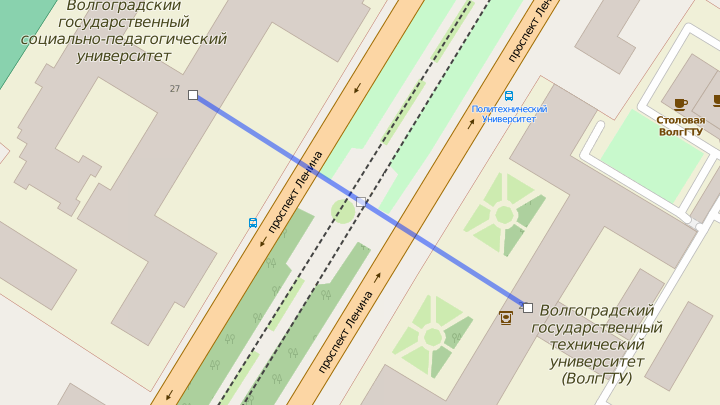
\includegraphics[width=\textwidth]{line}
    \end{figure}
\end{frame}

\subsection{Polyline}
\begin{frame}
    \frametitle{Polyline}
    \textbf{Полилиния (\emph{polyline})} -- это связанная последовательность 
    сегментов ...
    \begin{figure}[ht!]
        \center
        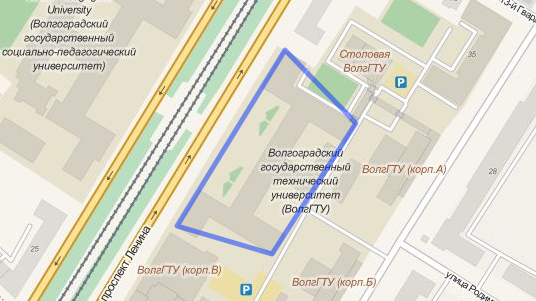
\includegraphics[width=\textwidth]{polyline}
    \end{figure}
\end{frame}

\begin{frame}
    \frametitle{Polyline}
    \begin{figure}[ht!]
        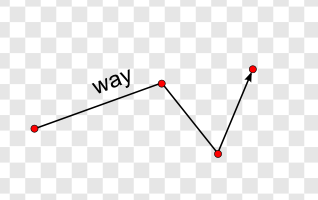
\includegraphics[width=0.5\textwidth]{p4}
        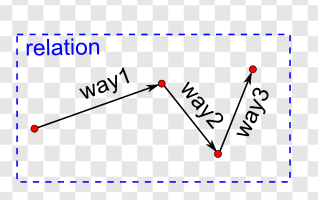
\includegraphics[width=0.5\textwidth]{p5}
    \end{figure}
    \begin{minipage}[h]{0.49\textwidth}
        \begin{figure}[ht!]
            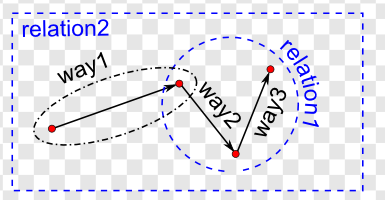
\includegraphics[width=\textwidth]{p6}
        \end{figure}
    \end{minipage}
    \scriptsize
    \begin{minipage}[h]{0.49\textwidth}
        \begin{enumerate}
            \item polyline = way(node1,node2,node3,node4);
            \item polyline = relation( way1(node1,node2),
                way2(node2,node3), way3(node3, node4) );
            \item polyline = relation2( way1(node1,node2), 
                relation1( way2(...), way3(...) ) )
        \end{enumerate}
    \end{minipage}
\end{frame}

\subsection{Polygon}
\begin{frame}
    \frametitle{Polygon}
    \textbf{Polygon (\emph{полигон})} -- это замкнутая полилиния, у которой 
    последняя точка совпадает с первой.
    \begin{figure}[ht!]
        \center
        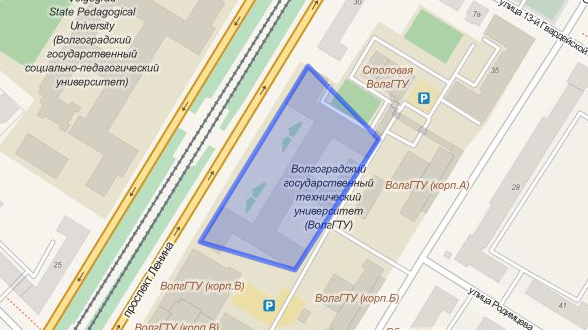
\includegraphics[width=\textwidth]{polygon}
    \end{figure}
\end{frame}

\begin{frame}
    \frametitle{Polygon}
    \begin{figure}[ht!]
        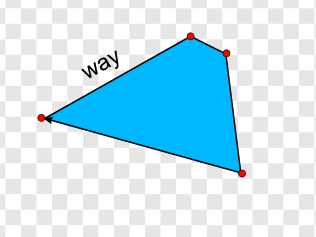
\includegraphics[width=0.5\textwidth]{p7}
        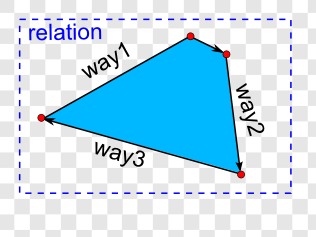
\includegraphics[width=0.5\textwidth]{p8}
    \end{figure}
    \begin{minipage}[h]{0.49\textwidth}
        \begin{figure}[ht!]
            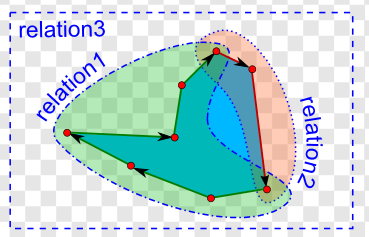
\includegraphics[width=\textwidth]{p9}
        \end{figure}
    \end{minipage}
    \scriptsize
    \begin{minipage}[h]{0.49\textwidth}
        \begin{enumerate}
            \item polygon = way(node1,node2,node3,node4,node1);
            \item polygon = relation( way1(node1,node2,node3), 
                way2(node3,node4), way3(node4,node1) );
            \item polygon = relation3( relation1(...), relation2(...) )
        \end{enumerate}
    \end{minipage}
\end{frame}

\subsection{Multipolygon}
\begin{frame}
    \frametitle{Multipolygon}
    \begin{figure}[ht!]
        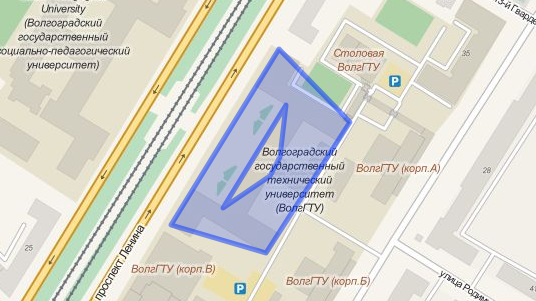
\includegraphics[width=\textwidth]{multipolygon_16x9}
    \end{figure}
\end{frame}

\begin{frame}[fragile]
    \frametitle{Multipolygon}
    \begin{lstlisting}
<node id='1' lat='48.71354' lon='44.52735' />
<node id='2' lat='48.71479' lon='44.52851' />
<node id='3' lat='48.71427' lon='44.52927' />
<node id='4' lat='48.71334' lon='44.52837' />
<node id='5' lat='48.71366' lon='44.52791' />
<node id='6' lat='48.71439' lon='44.52859' />
<node id='7' lat='48.71402' lon='44.52852' />
<node id='8' lat='48.71389' lon='44.52841' />
<way id='42'>
  <nd ref='1' /><nd ref='2' />
  <nd ref='3' /><nd ref='4' />
</way>
<way id='88'>
  <nd ref='5' /><nd ref='6' />
  <nd ref='7' /><nd ref='8' />
</way>
<relation id='1221'>
  <member type='way' ref='42' role='outer' />
  <member type='way' ref='88' role='inner' />
  <tag k='type' v='multipolygon' />
</relation>
    \end{lstlisting}
\end{frame}

\section{Сторонние инструменты}
\begin{frame}
    \frametitle{Сторонние инструменты}
    \begin{itemize}
        \item Leaflet (\url{http://leafletjs.com/})
        \item Mapnik (\url{http://mapnik.org/})
        \item Merkaartor (\url{http://merkaartor.be/})
        \item OSRM (\url{http://project-osrm.org/})
        \item ...\footnotemark
    \end{itemize}
    \begin{figure}[ht!]
        
\includegraphics[width=0.4\textwidth]{leaflet-logo}\quad
        
\includegraphics[width=0.4\textwidth]{mapnik-logo}
    \end{figure}
    \begin{figure}[ht!]
        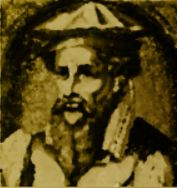
\includegraphics[width=0.2\textwidth]{merkaartor-logo}\quad
        
\includegraphics[width=0.4\textwidth]{osrm-logo}
    \end{figure}
    \footnotetext{\scriptsize\url{http://wiki.openstreetmap.org}}
\end{frame}

\section{Leaflet}
\begin{frame}
    \frametitle{Leaflet}
    \begin{figure}[ht!]
        
\includegraphics[width=0.4\textwidth]{leaflet-logo}
    \end{figure}
    \textbf{Leaflet}\footnotemark -- открытым проектом написаный на 
    JavaScript для отображения мобильных интерактивных карт.
    \footnotetext{\scriptsize\url{http://leafletjs.com/}}
    \begin{figure}[ht!]
        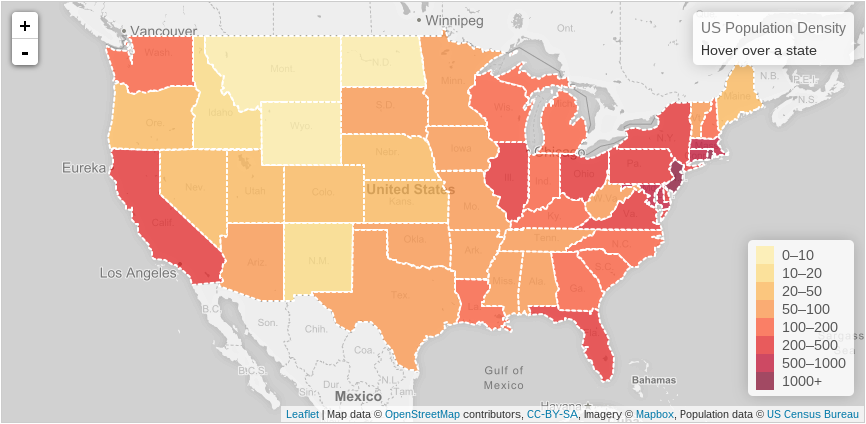
\includegraphics[width=0.7\textwidth]{leaflet-map-01}
        \footnotemark
    \end{figure}
    \footnotetext{\scriptsize\url{http://leafletjs.com/examples/choropleth.html}}
\end{frame}

\subsection{Примеры}
\begin{frame}[fragile]
    \frametitle{Leaflet}
    \begin{figure}[ht!]
        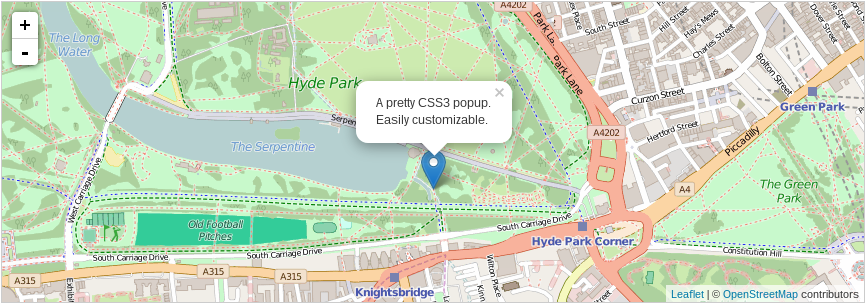
\includegraphics[width=\textwidth]{leaflet-map-02}
    \end{figure}
    \begin{lstlisting}[language=JavaScript]
var map = L.map('map').setView([51.505, -0.09], 13);

L.tileLayer('http://{s}.tile.osm.org/{z}/{x}/{y}.png', {
    attribution: '&copy; <a href=
        "http://osm.org/copyright">OpenStreetMap</a> contributors'
}).addTo(map);

L.marker([51.5, -0.09]).addTo(map)
    .bindPopup('A pretty CSS3 popup.<br> Easily customizable.')
    .openPopup();
    \end{lstlisting}
\end{frame}

\begin{frame}[fragile]
    \frametitle{Leaflet}
    \begin{figure}[ht!]
        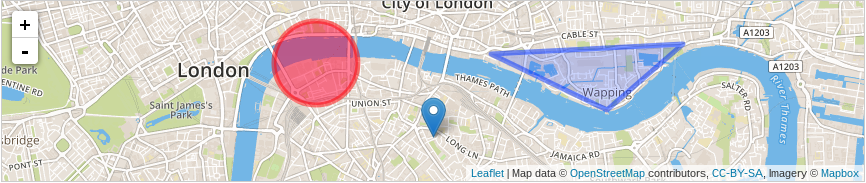
\includegraphics[width=\textwidth]{leaflet-map-03}
    \end{figure}
    \begin{lstlisting}[language=JavaScript]
var marker = L.marker([51.5, -0.09]).addTo(map);
var circle = L.circle([51.508, -0.11], 500, {
    color: 'red',
    fillColor: '#f03',
    fillOpacity: 0.5
}).addTo(map);
var polygon = L.polygon([
    [51.509, -0.08],
    [51.503, -0.06],
    [51.51, -0.047]
]).addTo(map);
    \end{lstlisting}
    \footnotemark{\scriptsize\url{http://leafletjs.com/examples/quick-start.html}}
\end{frame}

\begin{frame}
    \frametitle{GeoJSON}
    \begin{minipage}[h]{0.49\textwidth}
        Типы данных:
        \begin{itemize}
            \item Point
            \item MultiPoint
            \item LineString
            \item MultiLineString
            \item Polygon
            \item MultiPolygon
            \item GeometryCollection
        \end{itemize}
    \end{minipage}
    \begin{minipage}[h]{0.49\textwidth}
        Коллекции:
        \begin{itemize}
            \item Feature
            \item FeatureCollection
        \end{itemize}
    \end{minipage}
\end{frame}

\begin{frame}[fragile]
    \frametitle{GeoJSON}
    \begin{minipage}[h]{0.49\textwidth}
        \begin{lstlisting}
{
    "type": "Polygon",
    "coordinates": [[
        [44.52735, 48.71354],
        [44.52851, 48.71479],
        [44.52927, 48.71427],
        [44.52837, 48.71334],
        [44.52735, 48.71354]
    ],[
        [44.52791, 48.71366],
        [44.52859, 48.71439],
        [44.52852, 48.71402],
        [44.52841, 48.71389],
        [44.52791, 48.71366]
    ]]
}
        \end{lstlisting}
    \end{minipage}
    \begin{minipage}[h]{0.49\textwidth}
        \begin{figure}[ht!]
            \center
            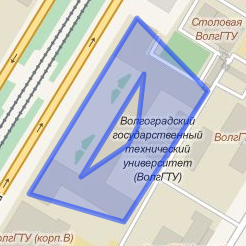
\includegraphics[width=\textwidth]{multipolygon_1x1}
        \end{figure}
    \end{minipage}
\end{frame}
\end{document}
